\documentclass{standalone}

\usepackage{standalone}
\usepackage{tikz}
\usetikzlibrary{calc,intersections}

\begin{document}
	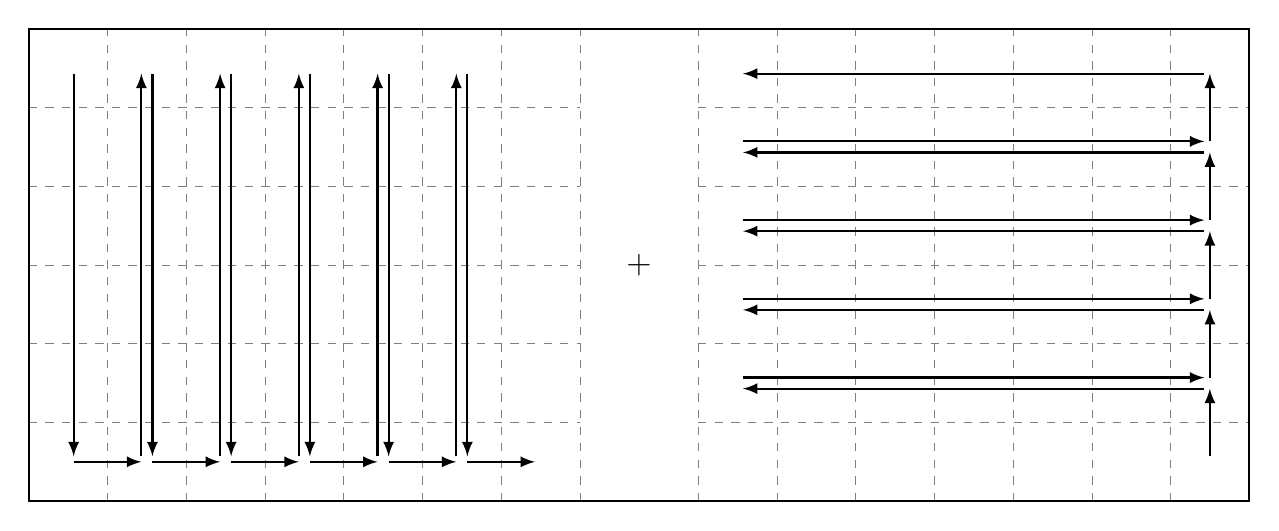
\begin{tikzpicture}
	
		\pgfmathtruncatemacro{\xsize}{7}
		\pgfmathtruncatemacro{\ysize}{6}


		\pgfmathsetmacro{\arrowoffset}{0.07}
		\pgfmathsetmacro{\intergriddistance}{1.5}
		
		% draw left grid
		\draw[dashed, very thin, black!50] (0,0) grid (\xsize, \ysize);
		% draw right grid
		\begin{scope}[shift = {({\xsize + \intergriddistance}, 0)}]
			\draw[dashed, very thin, black!50] (0,0) grid (\xsize, \ysize);
		\end{scope}
		
		\draw[thick] (0, 0) --
			(0, \ysize) --
			++(2 * \xsize + \intergriddistance, 0) --
			++(0, -\ysize) --
			cycle;

		\node at (\xsize + \intergriddistance / 2, \ysize / 2) {\large +};
		\pgfmathtruncatemacro{\xinnersize}{\xsize - 2}
		\pgfmathtruncatemacro{\yinnersize}{\ysize - 2}
		
		% draw in the left grid
		\begin{scope}[shift={(0.5, 0.5)}, thick]
			\foreach \col in {0, ..., \xinnersize}
			{
				\draw[-latex] (\col + \arrowoffset, \yinnersize - \arrowoffset + 1) -- (\col + \arrowoffset, \arrowoffset); % arrow down
				\ifnum\col<\xinnersize
					\draw[-latex] (\col + 1 - \arrowoffset, \arrowoffset) -- (\col + 1 - \arrowoffset, \yinnersize + 1 - \arrowoffset); % arrow up
				\fi

				\draw[-latex] (\col + \arrowoffset, 0) -- (\col + 1 - \arrowoffset, 0); % arrow right
			}
		% draw in the right grid
			\begin{scope}[shift = {({\xsize + \intergriddistance}, 0)}, thick]
				\foreach \row in {0, ..., \yinnersize}
				{
					\ifnum\row<\yinnersize
						\draw[-latex] (0 + \arrowoffset, \row + \arrowoffset + 1) -- (\xinnersize - \arrowoffset + 1, \row + \arrowoffset + 1); % arrow right
					\fi
					\draw[-latex] (\xinnersize - \arrowoffset + 1, \row - \arrowoffset + 1) -- (0 + \arrowoffset, \row - \arrowoffset + 1); % arrow left
					\draw[-latex] (\xinnersize + 1, \row + \arrowoffset) -- (\xinnersize + 1, \row + 1 -  \arrowoffset); % arrow up					
				}
			\end{scope}
		\end{scope}
	\end{tikzpicture}
\end{document}
